\documentclass[../mcmpaper]{subfiles}
\begin{document}
	\section{Problem 1:	Propagation Simulation Based on Yearly Time-Step Diffierence Equation}
	The parameters used in our analysis in this section are as the table(\Ref{table:chap3})
    \begin{table}
    \centering
    \caption{Key parameters for problem 1.}
    \label{table:chap3}
    \begin{tblr}{
      width=\linewidth,
      colspec={X[c]X[c]X[c]},
      hline{1, Z} = {2pt, solid},
      hline{2} = {solid}
    }
    a & b & c\\
    d & e & f
    \end{tblr}
    \end{table}
    \subsection{Method Overview}
    \begin{figure}[!ht]
    \centering
    \subfigure[The life cycle of the Asian giant hornet]{
       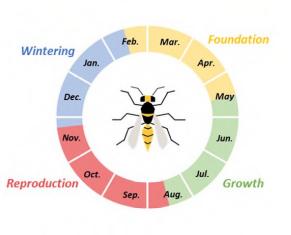
\includegraphics{3a}
    }
    \quad
	\subfigure[Parameter relationship in propagation simulation.]{
      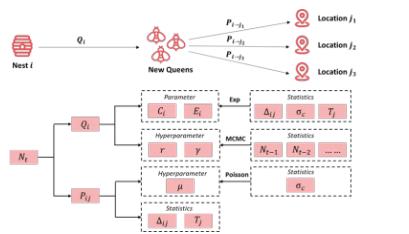
\includegraphics{3b}
      \label{second-b}
    }
    \caption{Introduction to pest extinction assessment model.}
    \label{fig:second}
    \end{figure}
    By clustering and plotting the existing positive data, we get that there are three nests near the State of Washington currently. Therefore, we set the initial number of nests to 3, and their location coordinates are the center of the latitude and longitude observed by citizens. We build a time-step difference equation [8] model in years to predict propagation. Based on the probability distribution of each parameter, we utilize Monte Carlo simulation to solve the model. The workflow is shown in Figure~\ref{second-b}.
    \subsection{Model Construction}
    Like other wasps, Asian giant hornets are an annual species, and the time points when queens produce male peak females are concentrated in September to November. Therefore, the life of the species has a strong periodicity, which belongs to rigid seasonal behaviour. This type of rigid seasonal behaviour is suitable for constructing a time-step difference equation, and iterating in units of years. In the annual Monte Carlo simulation, we conduct propagation on a single nest, and then calculate the number of nests each year.
    \paragraph{\itshape Parameters Selection.}
    When building the model, we select several parameters with practical significance such as biological populations and geographic conditions, which are introduced below.
    \par
    First of all, we consider the influence between nests. Since the Asian giant hornet will inevitably produce more nests when spreads in Washington State, the resources suitable for the species in State of Washington will gradually become scarce, and intraspecffic struggle will be inevitable. Therefore, we constructed a parameter to measure the competition for resources of different nests: the intra-species resource competition coeflcient $C_{ij}$, the formula is shown as follows:
    \end{document}
%%% Local Variables:
%%% mode: latex
%%% TeX-master: "../mcmpaper"
%%% End:
